\documentclass[12pt,letterpaper]{article}
\usepackage[T1]{fontenc}
\usepackage[utf8]{inputenc}
\usepackage[margin=1in]{geometry}
\usepackage{mathptmx}
\usepackage{microtype}
\usepackage{setspace}
\usepackage[authoryear,round]{natbib}
\usepackage[hidelinks]{hyperref}
\usepackage[most]{tcolorbox}
\setstretch{1.15}
\setlength{\parindent}{0pt}
\setlength{\parskip}{0.6em}
\setlength{\bibsep}{0.5em}
% Appendix table formatting
\usepackage{array}
\newcolumntype{C}[1]{>{\centering\arraybackslash}m{#1}}
\newcolumntype{R}[1]{>{\raggedleft\arraybackslash}m{#1}}
\usepackage{booktabs}
\usepackage{caption}
\usepackage{graphicx}
\usepackage{makecell}
\usepackage{pifont}
\usepackage[most]{tcolorbox}
\usepackage{xcolor}
\usepackage{amsmath}

\providecommand{\cmark}{\ding{51}}
\providecommand{\xmark}{\ding{55}}

\begin{document}
\begin{center}

{\Large\bfseries Calibrating LLM Agents for Theory-Grounded Social Simulation}
\end{center}

\section*{\normalsize Research Question and Scientific Opportunity}

Experiments provide an important foundation for testing theories of human behavior in organizational and social science, but conducting them at scale and across varied settings can be costly and time-consuming \citep{aher2023,ashokkumar2026}. These practical constraints limit opportunities to systematically examine how changes in information, incentives, and interaction structures affect human behaviors. Computational simulation offers a complementary means that has long helped researchers examine how individual decisions and interactions can produce collective outcomes within organizations \citep{davis2007}. In conventional agent-based models, researchers typically translate behavioral assumptions into explicit rules governing how agents use information and make choices. Drawing on patterns learned during training, large language models (LLMs) can generate potential behavioral responses from task descriptions and qualitative behavioral instructions \citep{manning2026}. For example, a model can be instructed to consider both personal earnings and inequality when choosing between monetary allocations, without requiring the researcher to specify a complete decision rule for that trade-off. 

Researchers have begun to explore this possibility by using LLMs to simulate human judgment and decision-making in social and behavioral research \citep{aher2023,argyle2023,filippas2024}. Applications include replicating established experiments \citep{aher2023}, constructing synthetic survey samples \citep{argyle2023}, exploring economic behavior under alternative conditions \citep{filippas2024}, and examining strategic interactions \citep{tranchero2026}. Recent work further examines whether simulations can predict human choices in novel environments and anticipate experimental treatment effects \citep{manning2026,ashokkumar2026}.

However, growing evidence raises concerns about the validity of using LLM-simulated responses to draw conclusions about human behavior. Successful replication in one setting does not establish that a model preserves the behavioral relationships needed for prediction in another \citep{manning2026}. Moreover, plausible aggregate responses can conceal insufficient heterogeneity, distorted associations among variables, and sensitivity to prompt wording or model updates \citep{bisbee2024,xie2026}. Even when simulated treatment effects correlate strongly with human effects, their magnitudes may be systematically overstated \citep{ashokkumar2026}. These discrepancies can also arise from how models interpret experimental instructions. \citet{gui2025} show that ambiguous prompts can lead LLMs to infer changes in unspecified features of an environment when researchers manipulate a treatment, undermining the intended experimental comparison. Such findings underscore the need to distinguish apparent human likeness from evidence that simulations support the particular behavioral inferences researchers seek to make \citep{gao2025,hullman2026}.

Researchers have sought to improve behavioral alignment by enriching both the characterization of simulated participants and the instructions governing their decisions. \citet{argyle2023} condition agents on demographic backstories, while \citet{park2026} incorporate interviews and prior survey responses to capture individual characteristics beyond demographic profiles. Focusing on how agents interpret decision environments, \citet{gui2025} clarify the experimental design through prompting to reduce unintended inferences about unspecified contextual features. \citet{manning2026} place behavioral theory at the center of agent construction, using theory-grounded instructions to generate candidate behaviors, calibrating agents against existing human observations, and evaluating their predictions in distinct environments. Their work provides an important foundation for connecting theoretically motivated agent behavior to empirical validation. Building on this foundation, we focus on two connected choices in agent construction: how a task is specified and which problem-solving strategies agents use to complete this task. This approach draws on the distinction between a problem space and the procedures operating within it \citep{simon1971}.

We examine whether theory-guided construction and calibration of LLM agent populations can improve the recovery of human behavioral relationships and support prediction beyond the calibration setting. We also examine whether calibration fit helps anticipate the performance of LLM simulation in new settings. To investigate these questions, we develop a three-stage framework.  The framework integrates theory-guided prompt generation, calibration using human data, and validation across experimental variants. Drawing on \citet{simon1971}, we ground this process in two components of human problem solving: how individuals represent a task and which problem-solving strategies they employ. We operationalize these components as Context Formation and Context Navigation, respectively, encoding them in prompts and calibrating a distribution over problem-solving strategies within a specified task representation. Our focal application is the observational-learning experiment of \citet{kremer2016}, in which consumers decide whether to purchase a product of uncertain quality. Waiting imposes a cost but can also signal quality because it reflects earlier purchase decisions, some made by informed consumers.

\section*{\normalsize Framework and AI Implementation}
The first stage generates prompts through Context Formation and Context Navigation. Context Formation establishes the task representation by specifying the agents, available information, feasible actions, and payoff structure. Its purpose is to make the experimental environment explicit while preserving the information available to each participant. In the \citet{kremer2016} setting, the task representation includes how previous purchases determine waiting time and whether earlier consumers may possess private information about product quality. Context Navigation specifies alternative problem-solving strategies within that task representation. Navigation prompts may differ, for example, in whether agents interpret earlier purchases as evidence of quality and how strongly they weigh that evidence against waiting costs. This distinction draws on \citeauthor{simon1971}'s (\citeyear{simon1971}) account of problem solving and allows heterogeneous problem-solving strategies within a shared, condition-appropriate task representation. Given the experimental materials and relevant behavioral theory, our automated procedure uses LLMs to generate formation prompts that establish the task representation and candidate navigation prompts that specify alternative problem-solving strategies. Generated formation prompts are checked against the experimental materials to ensure that they do not add information unavailable to human participants in the experiment or supply reasoning that those participants are expected to perform themselves.

The second stage calibrates the candidate population using human observations from a designated training condition. Following \citet{manning2026}, we generate responses from agents that share the applicable task representation but receive navigation prompts specifying different problem-solving strategies. We then estimate the nonnegative mixture weights of these strategies by minimizing the discrepancy between the mixture's predicted choices and observed human choices. These weights define a distribution over the candidate problem-solving strategies. Beyond estimating this distribution, we use training loss as an initial diagnostic for automated prompt selection. A high loss indicates that the calibrated candidate population fits the human training data poorly and motivates reviewing the candidate prompts. A low loss supports retaining the generated context formation and navigation prompts for further evaluation. We also examine whether training loss helps anticipate simulation performance in out-of-sample environments, treating it as a preliminary indicator rather than a substitute for external validation.

The third stage applies the calibrated distribution over problem-solving strategies to other decision settings without refitting the mixture weights. We adapt Context Formation to establish the task representation for the target environment, then sample navigation prompts according to the estimated weights. This procedure evaluates whether the calibrated distribution over problem-solving strategies retains predictive value across different task representations.

\section*{\normalsize Preliminary Evidence}
We empirically evaluate the proposed framework by comparing its ability to reproduce
human behavioral patterns against a baseline LLM agent that simulates each experimental
setting without Context Formation or Context Navigation. In the observational
learning experiment of \citet{kremer2016}, we estimate the optimized weights of the
navigation prompts using the high-informed-consumer condition (Q50) and evaluate the optimized prompt mixture on the low-informed-consumer condition (Q05) as an out-of-sample validation environment. We reproduce the directions and statistical significance of both focal hypotheses in the Q50--Q00 and Q05--Q00 comparisons. Uninformed consumers are less likely to purchase at short waiting times when informed consumers are present (H1), and the negative relationship between waiting time and purchasing is attenuated in their presence (H2). Replication in Q05 demonstrates transfer to a lower proportion of informed consumers without re-estimating the weights. In contrast, the baseline LLM agent produces estimated purchase probabilities approaching one at the shortest waiting time in both Q50 and Q00, reverses the signs of both hypothesis coefficients in the Q50--Q00 comparison, and fails to yield estimable hypothesis tests in the Q05--Q00 comparison. These results demonstrate improved recovery of the human behavioral relationships central to observational learning.

To extend this evidence beyond replication of published findings, we design a new experiment and generate simulation predictions before collecting human data. The experiment divides total waiting time into queuing time and shipping time. Queuing time refers to the delay generated by earlier consumers’ orders and can therefore signal product quality, while shipping time is an additional, randomly assigned delivery delay that imposes a cost without conveying quality information. We derive hypotheses from this distinction and first evaluate them through simulation, adapting the task representation while retaining the previously calibrated distribution over problem-solving strategies. Our framework produces results consistent with the hypothesized relationships, whereas baseline simulations without Context Formation and Context Navigation do not fully recover them. We subsequently conduct in-person experiments, finding support for the hypotheses and agreement with our framework’s predictions in the directions and statistical significance of the Q00–Q50 contrasts. By generating predictions for a newly designed experiment before collecting human data, we address concerns that successful replication reflects memorized findings or prompts tailored to reproduce known outcomes. The subsequent agreement with human behavior provides evidence of the framework’s ability to generalize beyond published experimental settings. Detailed procedures and results appear in the technical appendix.

Finally, we demonstrate that training loss serves as a quantitative diagnostic for prompt selection and out-of-sample performance. Holding the Context Formation fixed, we vary the candidate Context Navigation and calibrate their weights on the same human observations. The results reveal a progression from successful replication to partial replication and, ultimately, extreme behavioral patterns as training loss increases. Configurations with average training losses of 2.27 and 2.90 reproduce both hypotheses in both comparisons. At a loss of 6.20, replication becomes partial: H1 is no longer reproduced in the out-of-sample comparison. Configurations with losses of 6.23 and 7.43 generate extreme responses inconsistent with human behavioral variation, leaving the hypothesis tests non-estimable. In these configurations, the probit models encounter convergence or singularity problems, preventing reliable statistical inference. This pattern suggests that training loss provides a preliminary empirical criterion for selecting among calibrated candidate populations within a given task representation, reducing reliance on researchers' subjective judgment. Its association with subsequent replication success also supports its potential as an early indicator of out-of-sample simulation performance and generalizability (see technical Appendix).

\section*{\normalsize Development Plan and Expected Contribution}
This project develops Context Formation and Context Navigation as reusable research infrastructure for theoretically grounded and empirically validated social simulation. By distinguishing task representation from problem-solving strategies, the three-stage framework automates prompt generation, calibrates a distribution over strategies using human observations, and evaluates its transfer to alternative experimental settings. Our proof of concept reproduces the central observational-learning hypotheses of \citet{kremer2016}, where baseline simulations fail, and transfers the calibrated distribution to a newly designed in-person experiment without re-estimating its weights. The association between training loss and replication success in these initial tests further suggests a preliminary quantitative basis for selecting prompts and anticipating simulation failures. Together, these findings contribute a method for constructing and evaluating synthetic social systems through explicit links among behavioral theory, human evidence, and out-of-sample validation. We plan to extend the framework to a broader set of experiments involving organizationally relevant mechanisms, including social learning, strategic interaction, and coordination. This expansion will test whether the observed relationship between calibration fit and generalization persists across tasks and models, and identify conditions under which plausible task representations and problem-solving strategies remain insufficient. If successful, the framework would enable organizational scholars to investigate how behavioral relationships change across information structures and decision environments, use simulation evidence to prioritize new human experiments, and refine the boundary conditions of existing theories. Through these capabilities, it will contribute to more systematic and empirically grounded uses of LLM simulation in organizational research.

\clearpage
\begingroup
\singlespacing
\bibliographystyle{apalike}
\bibliography{references}
\endgroup

% ==================== Appendices ====================
\clearpage
\appendix

% Display section headings as "Appendix A: ..."
\renewcommand{\thesection}{Appendix \Alph{section}:}
\renewcommand{\thesubsection}{\Alph{section}.\arabic{subsection}}

% Number appendix tables and equations as A.1, B.1, etc.
\renewcommand{\thetable}{\Alph{section}.\arabic{table}}
\renewcommand{\theequation}{\Alph{section}.\arabic{equation}}

% ==================== Appendix A ====================
\section{Prompt Design}
\label{app:prompts}
\setcounter{table}{0}
\setcounter{equation}{0}

\subsection{Prompt Structure Comparison}
\label{app:prompt-designs}

% Number figures as A.1, A.2, etc.
\renewcommand{\thefigure}{\Alph{section}.\arabic{figure}}
\setcounter{figure}{0}

\begin{figure}[htbp]
    \centering
    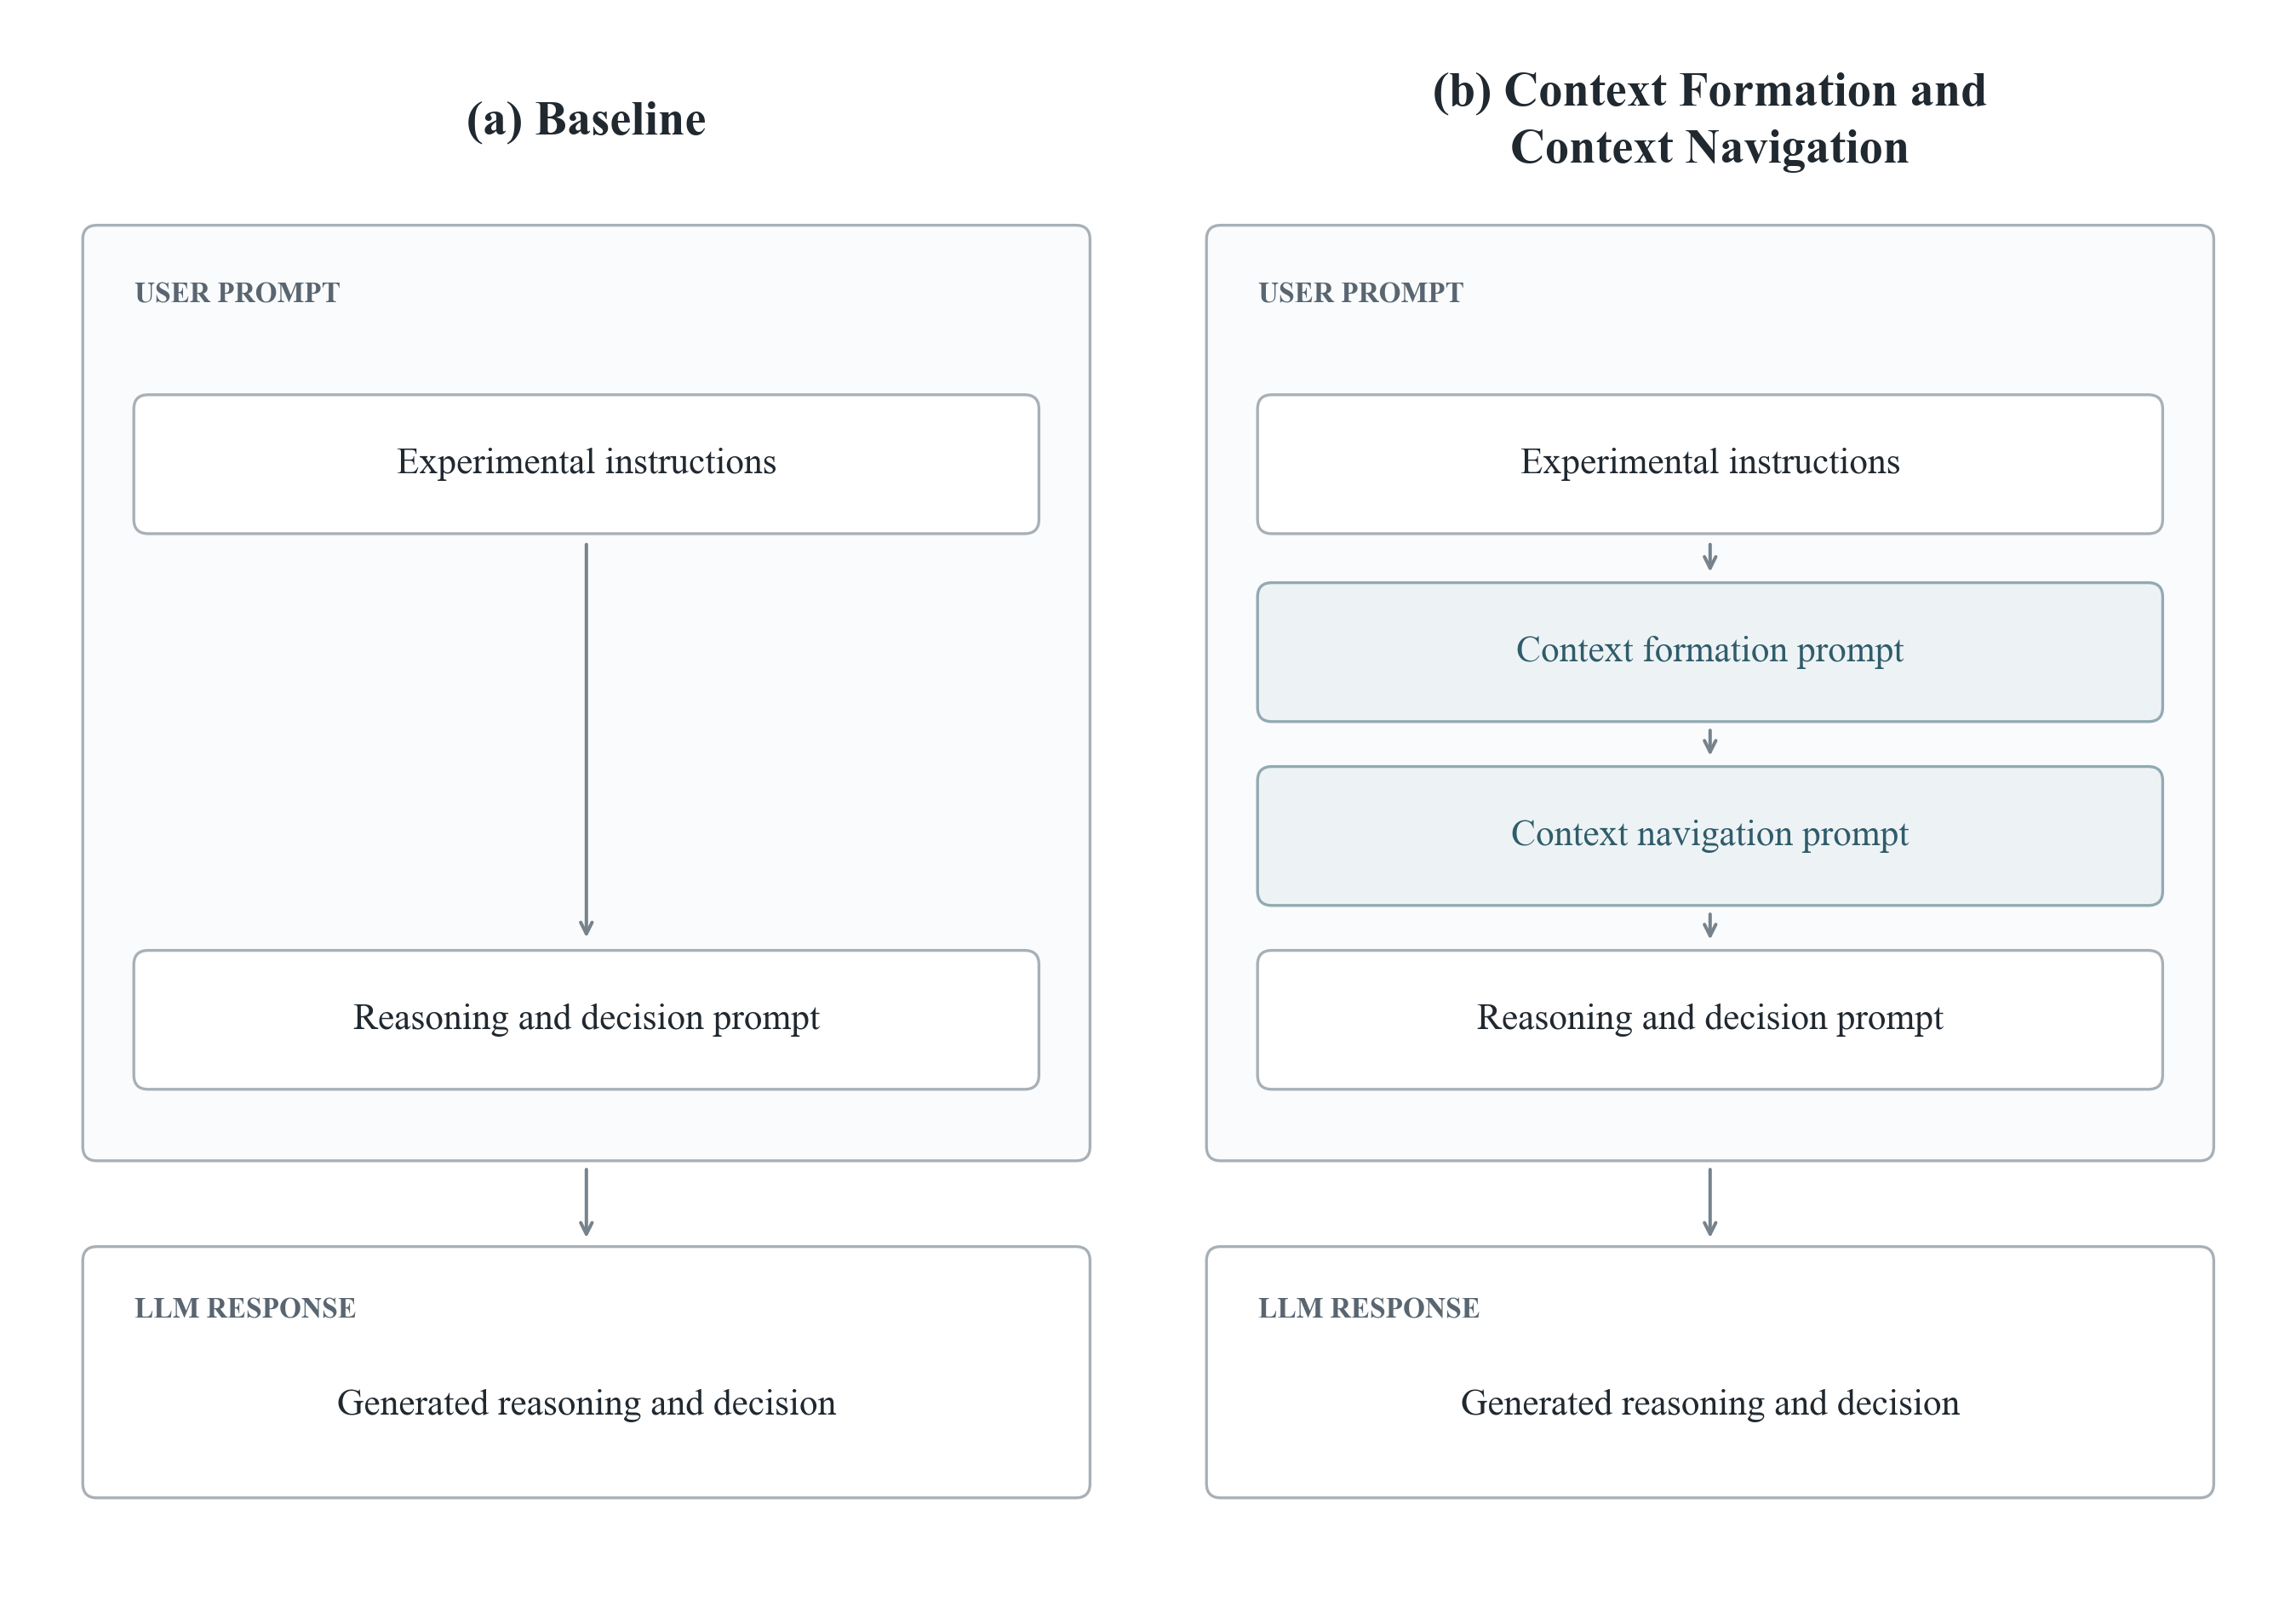
\includegraphics[width=\textwidth]{appendix-a-prompt-design.png}
    \caption{Prompt structures for the baseline and
    context formation and context navigation simulations}
    \label{fig:prompt-design}

    \smallskip
    \begin{minipage}{\textwidth}
        \footnotesize
        \textit{Note.} Arrows within each user prompt indicate
        the order of prompt components rather than separate
        conversational turns. The reasoning and decision prompt
        requests chain-of-thought (CoT) reasoning and a final
        decision.
    \end{minipage}
\end{figure}

\subsection{Context Formation and Context Navigation Examples}

The following box presents a sample context formation prompt for
the Q50 condition in Kremer and Debo (2016). The Q00 condition uses
a different context formation prompt to reflect its distinct
information environment, in which no consumers are informed,
compared with 50\% in Q50.

\begin{tcolorbox}[
    colback=white,
    colframe=black,
    colbacktitle=white,
    coltitle=black,
    boxrule=0.5pt,
    arc=2mm,
    left=3mm,
    right=3mm,
    top=2mm,
    bottom=2mm,
    fonttitle=\large\bfseries,
    title={Context Formation for
        \textcolor{red!70!black}{Kremer and Debo (2016)}}
]
\ttfamily
In sum, you are a consumer participating in a repeated market experiment in which you decide in each round whether to order a product from a firm under uncertainty about its value and with a delay before delivery.

In each round, you are part of a fixed group of 4 consumers, and the experiment consists of multiple independent rounds (26 in total). At the start of every round, the product's quality (high or low) is randomly determined and remains the same for all consumers in that round. Your consumer type (informed or uninformed) is also randomly assigned each round, and the fraction of informed consumers and the prior probability of high quality are fixed parameters of the environment and common knowledge.

All consumers arrive in a random, unobservable order. When you arrive, you are quoted a wait time that equals the number of prior consumers who chose to order plus one, which determines both your delivery delay and your waiting cost. You do not observe how many consumers arrived before you or their decisions directly; all interaction occurs indirectly through the wait time. The firm is non-strategic and follows a fixed rule: it produces one unit per week and delivers in first-in-first-out order after all decisions are made.

Within each round, the sequence is: product quality and consumer types are realized → consumers arrive in random order → each consumer observes a wait time and makes a one-time decision to order or not → after all decisions, production and delivery occur. Decisions cannot be revised. The \$4 endowment is reset each round, and earnings accumulate across rounds. You also have access to information from past rounds (e.g., wait times, types, decisions, and outcomes), but each round is otherwise independent.

\end{tcolorbox}

We identify behavioral mechanisms from the target experimental
paper and express each mechanism as a single sentence in the
context navigation prompt. Each mechanism is assigned one of two
contrasting behavioral settings. In the example below, the two
mechanisms concern risk preferences (risk avoidance versus risk
seeking) and learning from earlier consumers' behavior (limited
versus substantial consideration). Combining these binary settings
yields four context navigation candidates, each containing one
sentence per mechanism. For each API call, a single candidate is
selected according to the optimized selection weights and included
in the prompt.

\begin{tcolorbox}[
    colback=white,
    colframe=black,
    colbacktitle=white,
    coltitle=black,
    boxrule=0.5pt,
    arc=2mm,
    left=3mm,
    right=3mm,
    top=2mm,
    bottom=2mm,
    fonttitle=\large\bfseries,
    title={Context Navigation Candidates for
        \textcolor{red!70!black}{Kremer and Debo (2016)}}
]
\ttfamily
\begin{enumerate}
    \renewcommand{\labelenumi}{\arabic{enumi}.}
    \setlength{\itemsep}{\baselineskip}
    \setlength{\parsep}{0pt}

    \item You tend to avoid risky options, preferring choices with more certain outcomes even when they may offer lower potential rewards. You give little consideration to earlier consumers' behavior as a potential source of evidence, making no use of the rules of the decision environment to determine whether their decisions are informative about what you observe and placing little weight on any resulting implication.

    \item You tend to avoid risky options, preferring choices with more certain outcomes even when they may offer lower potential rewards. You give significant consideration to earlier consumers' behavior as a potential source of evidence, using the rules of the decision environment to determine whether their decisions are informative about what you observe and placing substantial weight on any resulting implication.

    \item You tend to favor risky options, accepting greater uncertainty in pursuit of higher potential rewards. You give little consideration to earlier consumers' behavior as a potential source of evidence, making no use of the rules of the decision environment to determine whether their decisions are informative about what you observe and placing little weight on any resulting implication.

    \item You tend to favor risky options, accepting greater uncertainty in pursuit of higher potential rewards. You give significant consideration to earlier consumers' behavior as a potential source of evidence, using the rules of the decision environment to determine whether their decisions are informative about what you observe and placing substantial weight on any resulting implication.
\end{enumerate}
\end{tcolorbox}

% ==================== Appendix B ====================
\clearpage
\section{Comparison of Experimental and Simulation Results}
\label{app:results}
\setcounter{table}{0}
\renewcommand{\thetable}{\Alph{section}.\arabic{table}}

% -------------------- Q50 versus Q00 --------------------
\vspace*{6pt}
\begingroup
\setstretch{1}
\renewcommand{\arraystretch}{1.15}
\setlength{\extrarowheight}{0pt}
\setlength{\tabcolsep}{6pt}
\centering

\captionof{table}{Human and LLM Replication Results of Q50 \& Q00 Condition (Kremer \& Debo, 2016)}
\label{tab:q50q00}

\resizebox{\textwidth}{!}{%
\begin{tabular}{
    l
    C{2.4em}
    C{2.4em}
    R{3.8em}
    R{3.8em}
    C{6em}
    C{3.8em}
    R{3.8em}
    R{3.8em}
    C{6em}
}
\toprule
\multicolumn{1}{c}{}
& \multicolumn{5}{c}{\textbf{Hypothesis 1}}
& \multicolumn{4}{c}{\textbf{Hypothesis 2}} \\
\cmidrule(lr){2-6}
\cmidrule(lr){7-10}
\textbf{Paper/Prompt Design}
& Q00
& Q50
& $\chi^2$
& $p$-value
& \textbf{Conclusion}
& $\beta_3$
& $\chi^2$
& $p$-value
& \textbf{Conclusion} \\
\midrule
Kremer and Debo (2016)
& \makecell{95\%}
& \makecell{68\%}
& 31.23
& $<0.01$
& \makecell{--}
& \makecell{0.85}
& 74.34
& $<0.01$
& \makecell{--} \\
Baseline
& \makecell{100\%}
& \makecell{100\%}
& \makecell{--}
& \makecell{--}
& \makecell{\xmark}
& \makecell{--}
& \makecell{--}
& \makecell{--}
& \makecell{\xmark} \\
Context Formation \& Context Navigation
& \makecell{97\%}
& \makecell{80\%}
& 32.96
& $<0.01$
& \makecell{\cmark}
& \makecell{2.04}
& 121.04
& $<0.01$
& \makecell{\cmark} \\
\bottomrule
\end{tabular}%
}

\vspace{0.5em}
\parbox{\textwidth}{%
\footnotesize
\textit{Note.}
Statistics are reported as ``--'' when the regression is not estimable because the prompt design produces perfect or near-perfect prediction. In this setting, perfect prediction implies that decisions do not differ across the two condition. These entries therefore indicate replication failure.
}
\par
\endgroup

% -------------------- Q05 versus Q00 --------------------
\vspace*{6pt}
\begingroup
\setstretch{1}
\renewcommand{\arraystretch}{1.15}
\setlength{\extrarowheight}{0pt}
\setlength{\tabcolsep}{6pt}
\centering

\captionof{table}{Human and LLM Replication Results of Q05 \& Q00 Condition (Kremer \& Debo, 2016)}
\label{tab:q05q00}

\resizebox{\textwidth}{!}{%
\begin{tabular}{
    l
    C{2.4em}
    C{2.4em}
    R{3.8em}
    R{3.8em}
    C{6em}
    C{3.8em}
    R{3.8em}
    R{3.8em}
    C{6em}
}
\toprule
\multicolumn{1}{c}{}
& \multicolumn{5}{c}{\textbf{Hypothesis 1}}
& \multicolumn{4}{c}{\textbf{Hypothesis 2}} \\
\cmidrule(lr){2-6}
\cmidrule(lr){7-10}
\textbf{Paper/Prompt Design}
& Q00
& Q05
& $\chi^2$
& $p$-value
& \textbf{Conclusion}
& $\beta_3$
& $\chi^2$
& $p$-value
& \textbf{Conclusion} \\
\midrule
Kremer and Debo (2016)
& \makecell{95\%}
& \makecell{72\%}
& 18.41
& $<0.01$
& \makecell{--}
& \makecell{0.47}
& 21.12
& $<0.01$
& \makecell{--} \\
Baseline
& \makecell{--}
& \makecell{--}
& \makecell{--}
& \makecell{--}
& \makecell{\xmark}
& \makecell{--}
& \makecell{--}
& \makecell{--}
& \makecell{\xmark} \\
Context Formation \& Context Navigation
& \makecell{97\%}
& \makecell{85\%}
& 19.94
& $<0.01$
& \makecell{\cmark}
& \makecell{1.81}
& 95.02
& $<0.01$
& \makecell{\cmark} \\
\bottomrule
\end{tabular}%
}

\vspace{0.5em}
\parbox{\textwidth}{%
\footnotesize
\textit{Note.} Baseline statistics are reported as ``--'' because
the regression failed with singular-matrix errors, leaving no
valid coefficient estimates or hypothesis tests available.
Successful replication therefore cannot be established.
}
\par
\endgroup


% ==================== Appendix C ====================
\clearpage
\section{Wait-Time Decomposition Experiment}
\label{app:wait-time-decomposition}

\setcounter{table}{0}
\setcounter{equation}{0}
\renewcommand{\thetable}{\Alph{section}.\arabic{table}}
\renewcommand{\theequation}{\Alph{section}.\arabic{equation}}

% ==================== C.1 ====================
\subsection{In-Person Experimental Design}
\label{app:decomposition-design}

We designed the \textit{wait-time decomposition variant} of
Kremer and Debo's (2016) original experiment to evaluate
predictions in a novel setting before collecting human data.

Unlike the original design, this variant decomposes total
waiting time into queuing time and shipping time. Shipping time
is designed to represent a pure waiting cost, whereas queuing
time may additionally convey information about product quality
through earlier consumers' purchase decisions. Comparing Q50,
where 50\% of consumers are informed, with Q00, where no consumers
are informed, allows us to examine responses to the informational
content of waiting beyond its total cost.

% ==================== C.2 ====================
\subsection{Hypotheses and Regression Specification}
\label{app:decomposition-specification}

Before conducting simulations or collecting human data, we
derived two hypotheses from the experimental design. To evaluate
these hypotheses in both simulated and human data, we use a
pooled linear probability model estimated by ordinary least
squares (OLS), allowing the slopes of queuing time, rank, and
total waiting time to differ between Q00 and Q50:
\begin{equation}
\begin{aligned}
Y_{it}
={}& \alpha + \tau T_i
   + b_q q_{it} + \gamma_q T_i q_{it} \\
 & + b_r r_{it} + \gamma_r T_i r_{it}
   + b_d d_{it} + \gamma_d T_i d_{it}
   + \varepsilon_{it}.
\end{aligned}
\label{eq:decomposition-model}
\end{equation}

Here, $Y_{it}$ equals one if participant $i$ purchases in round
$t$ and zero otherwise. The treatment indicator $T_i$ equals
one for Q50 and zero for Q00. Queuing time is denoted by
$q_{it}$, shipping time by $s_{it}$, total waiting time by
$d_{it}=q_{it}+s_{it}$, and arrival rank by $r_{it}$.
The coefficients $b_q$, $b_r$, and $b_d$ are the Q00 slopes;
$\gamma_q$, $\gamma_r$, and $\gamma_d$ are the corresponding
Q50-minus-Q00 slope differences.

\paragraph{H1: Waiting composition and positive purchase signals.}
Holding arrival rank and total waiting time fixed, replacing
one unit of shipping time with one unit of queuing time should
increase purchase probability in Q50. The composition slope
should also be more positive in Q50 than in Q00, while the Q00
slope is predicted to be negligible:
\begin{equation}
b_q+\gamma_q>0,
\qquad
\gamma_q>0,
\qquad
b_q\approx 0.
\label{eq:decomposition-h1}
\end{equation}
At a fixed rank, more earlier purchases also imply fewer earlier
nonpurchases.

\paragraph{H2: Rank and negative nonpurchase signals.}
Holding queuing time and shipping time fixed, a higher arrival
rank should reduce purchase probability in Q50. The rank slope
should also be more negative in Q50 than in Q00, while the Q00
slope is predicted to be negligible:
\begin{equation}
b_r+\gamma_r<0,
\qquad
\gamma_r<0,
\qquad
b_r\approx 0.
\label{eq:decomposition-h2}
\end{equation}
Given the mapping from earlier purchases to queuing time,
a higher rank at fixed queuing time corresponds to more earlier
nonpurchases.

% ==================== C.3 ====================
\subsection{Simulation Predictions and Subsequent Human Validation}
\label{app:decomposition-results}

We first evaluated these hypotheses using baseline simulations
and simulations with Context Formation and Context Navigation.
For the latter, we adapted the task representation while retaining
the previously calibrated distribution over problem-solving
strategies. We subsequently conducted an in-person experiment at
The Chinese University of Hong Kong (CUHK) with 100 participants,
organized into groups of four, each completing 25 rounds of
decisions. Tables~\ref{tab:decomposition-h1}
and~\ref{tab:decomposition-h2} compare the simulation predictions
with the
subsequently collected human results. Coefficients are expressed
in percentage points.

% -------------------- H1 table --------------------
\begin{table}[htbp]
\centering
\begingroup
\setstretch{1}
\renewcommand{\arraystretch}{1.15}
\setlength{\tabcolsep}{6pt}

\caption{H1: Waiting Composition Effects in Human and
LLM Simulation Data}
\label{tab:decomposition-h1}

\resizebox{\textwidth}{!}{%
\begin{tabular}{lrrrrrr}
\toprule
& \multicolumn{2}{c}{\textbf{Q00}}
& \multicolumn{2}{c}{\textbf{Q50}}
& \multicolumn{2}{c}{\textbf{Q50 $-$ Q00}} \\
\cmidrule(lr){2-3}
\cmidrule(lr){4-5}
\cmidrule(lr){6-7}
\textbf{Data/Prompt Design}
& $b_q$ & $p$-value
& $b_q+\gamma_q$ & $p$-value
& $\gamma_q$ & $p$-value \\
\midrule
Human
& $-9.20$ & $0.068$
& $24.00$ & $<0.001$
& $33.19$ & $<0.001$ \\
Baseline
& $-22.67$ & $<0.001$
& $5.16$ & $0.028$
& $27.83$ & $<0.001$ \\
\makecell[l]{Context Formation \& Context Navigation}
& $1.61$ & $0.593$
& $16.38$ & $<0.001$
& $14.77$ & $<0.001$ \\
\bottomrule
\end{tabular}%
}

\medskip
\begin{minipage}{\textwidth}
\footnotesize
\textit{Note.} Coefficients are expressed in percentage points
and represent the change in purchase probability associated
with replacing one unit of shipping time with one unit of
queuing time, holding rank and total waiting time fixed.
\end{minipage}

\endgroup
\end{table}

% -------------------- H2 table --------------------
\begin{table}[htbp]
\centering
\begingroup
\setstretch{1}
\renewcommand{\arraystretch}{1.15}
\setlength{\tabcolsep}{6pt}

\caption{H2: Arrival Rank Effects in Human and
LLM Simulation Data}
\label{tab:decomposition-h2}

\resizebox{\textwidth}{!}{%
\begin{tabular}{lrrrrrr}
\toprule
& \multicolumn{2}{c}{\textbf{Q00}}
& \multicolumn{2}{c}{\textbf{Q50}}
& \multicolumn{2}{c}{\textbf{Q50 $-$ Q00}} \\
\cmidrule(lr){2-3}
\cmidrule(lr){4-5}
\cmidrule(lr){6-7}
\textbf{Data/Prompt Design}
& $b_r$ & $p$-value
& $b_r+\gamma_r$ & $p$-value
& $\gamma_r$ & $p$-value \\
\midrule
Human
& $-3.16$ & $0.300$
& $-17.97$ & $<0.001$
& $-14.81$ & $<0.001$ \\
Baseline
& $9.06$ & $<0.001$
& $-5.44$ & $<0.001$
& $-14.51$ & $<0.001$ \\
\makecell[l]{Context Formation \& Context Navigation}
& $-0.56$ & $0.677$
& $-6.96$ & $<0.001$
& $-6.40$ & $0.002$ \\
\bottomrule
\end{tabular}%
}

\medskip
\begin{minipage}{\textwidth}
\footnotesize
\textit{Note.} Coefficients are expressed in percentage points
and represent the change in purchase probability associated
with a one-unit increase in arrival rank, holding queuing time
and shipping time fixed.
\end{minipage}

\endgroup
\end{table}

The simulations with Context Formation and Context Navigation
produce the predicted signs and statistical significance for
the Q50 slopes and Q50-minus-Q00 slope differences, alongside
Q00 coefficients that are not statistically distinguishable
from zero. The baseline recovers the Q50 slopes and
between-condition differences but produces significantly
nonzero Q00 coefficients, failing to recover the full
hypothesized pattern. The subsequent human experiment supports
the predicted Q50 effects and between-condition differences,
with Q00 coefficients also not statistically distinguishable
from zero at the 5\% level. Because the simulation predictions
preceded human data collection, they could not have been
tailored to or memorized these experimental outcomes. 

% ==================== Appendix D ====================
\clearpage
\section{Training Loss and Hypothesis Outcomes}
\label{app:training-loss}

\setcounter{figure}{0}
\renewcommand{\thefigure}{\Alph{section}.\arabic{figure}}

% Before uploading, correct the image label
% M1,M2,M4 to M1,M3,M4 to match the mechanism definitions below.

\begin{figure}[htbp]
    \centering
    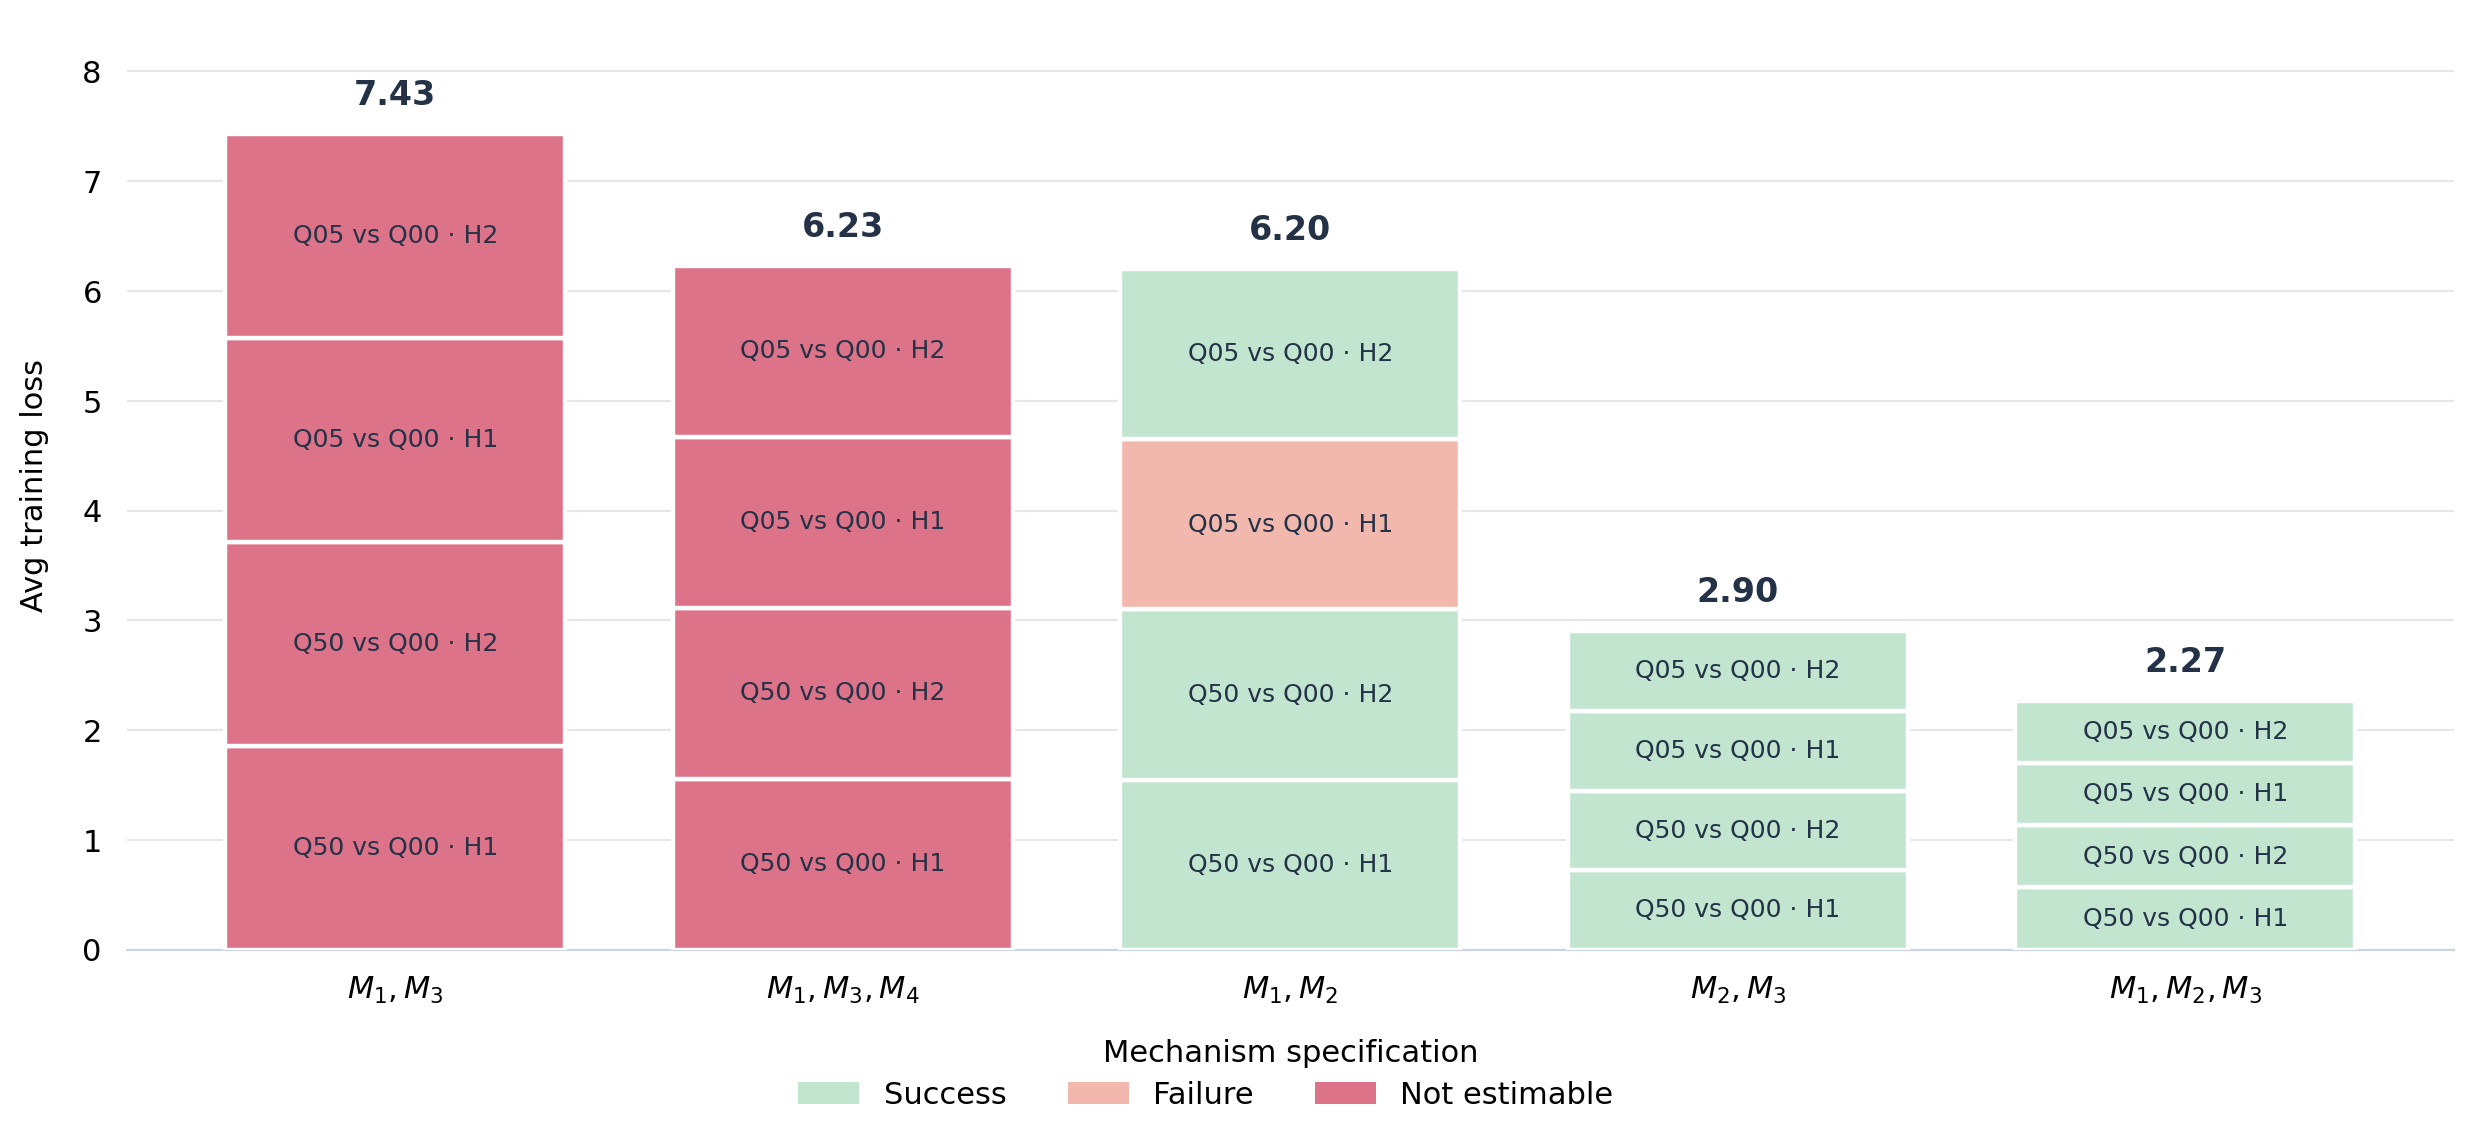
\includegraphics[width=\textwidth]{results_vis.png}
    \caption{Average training loss and hypothesis outcomes
    across navigation mechanism specifications}
    \label{fig:training-loss}

    \smallskip
    \begin{minipage}{\textwidth}
        \footnotesize
        \textit{Note.} Average training loss is the mean binary
        cross-entropy between observed human purchase decisions
        and predictions obtained by weighting navigation
        candidates' simulated decisions using the fitted selection
        weights. It is calculated over 875 Q50 training observations;
        lower values indicate better training fit.

        \smallskip
        The horizontal axis identifies the included mechanisms:
        $M_1$ denotes cost--benefit evaluation;
        $M_2$, risk preferences;
        $M_3$, social learning from earlier consumers' behavior;
        and $M_4$, choice consistency.
        Each mechanism has two contrasting behavioral settings,
        yielding four candidates for two mechanisms and eight
        candidates for three mechanisms.

        \smallskip
        Total bar height represents average training loss.
        The four equal sections indicate hypothesis outcomes,
        not separate loss components. Green indicates successful
        replication, light red indicates failure, and dark red
        indicates that the relevant test is not estimable.
    \end{minipage}
\end{figure}


\end{document}
